\documentclass[fleqn]{rbfin}

%%%%%%%%%%%%%%%%%%%%%%%%%%%%%%%%%%%%
% BEGIN DOCUMENT
%%%%%%%%%%%%%%%%%%%%%%%%%%%%%%%%%%%%
\begin{document}
% Para artigos em PORTUGUÊS, alterar a linha abaixo para \selectlanguage{brazil}
\selectlanguage{english}
\frenchspacing

%%%%%%%%%%%%%%%%%%%%%%%%%%%%%%%%%%%%
% FRONT MATTER
%%%%%%%%%%%%%%%%%%%%%%%%%%%%%%%%%%%%

% ARTICLE TITLE
\title{Brazilian Review of Finance: A Template} % Appears on title page

% ARTICLE SHORT TITLE
\shorttitle{BRF: A Template} % appears on header every other page

% RELEVANT DATES
\nota{Submitted on December 14, 2024.
%
% Revised on May 25, 2024.
% %
% Accepted on June 9, 2024.
% %
% Published online in January 2024.
% %
% Editor in charge: Mr.\ Editor.
}

% AUTHOR INFORMATION
\author{\centering
% Define affiliations
\affiliations{1}{University of Victoria}
\affiliations{2}{ECE 503 Optimization for Machine Learning}
% AUTHOR 1
\textbf{Wang Daming}%
\email{wdm1732418365@gmail.com}
\affiliationlink{1} % Match with the affiliations defined above
% \orcidlink{0000-0000-0000}
\and % separate authors with \and
% % AUTHOR 2
% \textbf{Author Two}%
% \email{author.two@email}
% \affiliationlink{2} % Match with the affiliations defined above
% \orcidlink{0000-0000-0000}
% \and
% % AUTHOR 3
% \textbf{Author Three}%
% \email{author.three@email}
% \affiliationlink{1} % Match with the affiliations defined above
% \affiliationlink{2} % Match with the affiliations defined above
% \orcidlink{0000-0000-0000}
% AND SO ON...
\\[20pt]
% Print the affiliations:
\affiliationname{1}
\affiliationname{2}
}
\autor{Daming Wang, 2024} % appears on header every other page

% JOURNAL INFO
\maketitle
% \pagina{1}
% \rbfd{
% \href
% {http://bibliotecadigital.fgv.br/ojs/index.php/rbfin/index}
% {Revista Brasileira de Finanças (Online)}
% % {Brazilian Review of Finance (Online)},
% Rio de Janeiro,
% \textcolor{BrickRed}{Vol. XX,}
% \textcolor{BrickRed}{No. Y,}
% \textcolor{BrickRed}{August 2024,}
% \textcolor{BrickRed}{pp. x--xx}
% \qquad ISSN 1679-0731, ISSN online 1984-5146}
% \rbfc{\copyright
% 2024
% \href
% {https://www.sbfin.org.br}
% {Sociedade Brasileira de Finanças},
% under a
% \href
% {https://creativecommons.org/licenses/by/4.0/}
% {Creative Commons Attribution 4.0 license} 
% \quad\url{https://doi.org/10.xxxx/xxxxxxxx}
% }
% \rbfe{
% \href
% {http://bibliotecadigital.fgv.br/ojs/index.php/rbfin/index}
% % {Brazilian Review of Finance (Online)}
% {Revista Brasileira de Finanças (Online)}
% XX(Y),
% 2024
% }

% ABSTRACT, KEYWORDS AND JEL
\begin{abstract}
\myabstract{%
% ABSTRACT
Your abstract goes here! \lipsum[1-1]
}

% KEYWORDS (separated by semicolon)
\keywordslist{Risk measures; Standard deviation.}

% JEL CODES (separated by colon)
% \jelcodeslist{E3, C41, C43.}
\end{abstract}

%%%%%%%%%%%%%%%%%%%%%%%%%%%%%%%%%%%%
% END OF FRONT MATTER
%%%%%%%%%%%%%%%%%%%%%%%%%%%%%%%%%%%%

%%%%%%%%%%%%%%%%%%%%%%%%%%%%%%%%%%%%
% DOCUMENT MAIN SECTIONS
%%%%%%%%%%%%%%%%%%%%%%%%%%%%%%%%%%%%
\section{Introduction}\label{sec-intro}

Below you can find a scheme of citation commands and corresponding outputs. You can also cite multiple references with a single \lstinline[language=TeX]/\cite/ command; for instance, \lstinline[language=TeX]/\citep{markowitz52,rockafellar02,rockafellar06}/ produces the output \citep{markowitz52,rockafellar02,rockafellar06}.  \lipsum[][1-21]

\begin{table}[ht]
\begin{center}
\begin{tabular}{L{6cm}r}
\lstinline[language=TeX]/\citet{markowitz52}/ & \citet{markowitz52}\tabularnewline
\lstinline[language=TeX]/\citep[p.9]{markowitz52}/ & \citep[p.9]{markowitz52}\tabularnewline
\lstinline[language=TeX]/\citename{markowitz52}/ & \citename{markowitz52}\tabularnewline
\lstinline[language=TeX]/\citeyear*{markowitz52}/ & \citeyear*{markowitz52}\tabularnewline
\lstinline[language=TeX]/\citeyear{markowitz52}/ & \citeyear{markowitz52}
\end{tabular}
\end{center}
\end{table}

In the \hyperref[refs]{References} section, you can make the title of a reference \emph{clickable} by including the \lstinline/doi/ field in the \lstinline/references.bib/ file, as shown in the example below. In practice, the \lstinline/doi/ field accepts any type of web address; this can be useful when you have a reference which has no DOI but does have a permalink. Additionally, if you want to explicitly display the URL for a given reference, then just add the \lstinline/url/ field in the \lstinline/bib/ file. These possibilities are illustrated in the \hyperref[refs]{References} section.
\begin{lstlisting}[language=TeX]
@article{rockafellar02,
title={Conditional value-at-risk for general loss distributions},
author={Rockafellar, R Tyrrell and Uryasev, Stanislav},
journal={Journal of banking \& finance},
volume={26},
number={7},
pages={1443--1471},
year={2002},
doi = {https://doi.org/10.1016/S0378-4266(02)00271-6},
}
\end{lstlisting}

\subsection{Useful tools for reference managing}
There are several useful tools to help organize your references. Here are some of them:
\begin{enumerate}[label=(\roman*), noitemsep]
\item \url{https://www.mendeley.com}
\item \url{https://www.jabref.org}
\item \url{https://www.zotero.org/}
\item \url{https://truben.no/latex/bibtex/}
\end{enumerate}

\section{Methodology}
In this section you should discuss the methodology.\footnote{Footnote links should come after punctuation.}

\subsection{Figures}
Figure~\ref{fig1} was generated in \lstinline/R/ through the following code:
\begin{lstlisting}[language=R]
x = seq(from=0, to=2*pi, length=100)
cm = 1/2.54 # this is just for defining units of measurement
pdf(file='plot.pdf', width=9*cm, height=7*cm, bg=rgb(0,0,0,.1))
par(mai = c(2*cm,1*cm,.5*cm,1*cm))
plot(x, sin(x), type ='l')
dev.off()
\end{lstlisting}

\begin{figure}[ht]
\begin{center}
\caption{A figure}\label{fig1}
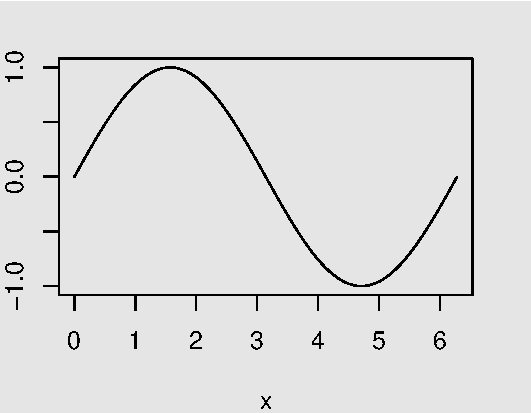
\includegraphics{media/plot.pdf}
\end{center}
\end{figure}

Ideally, the dimensions of the figure should be controlled \emph{outside} of \LaTeX, as the preceding \lstinline/R/ code illustrates. If you cannot generate or obtain the figure with appropriate sizing, then adding the optional argument \lstinline/[width=9cm]/ to the \lstinline/\includegraphics/ command will do the job. Below we illustrate usage of the \lstinline!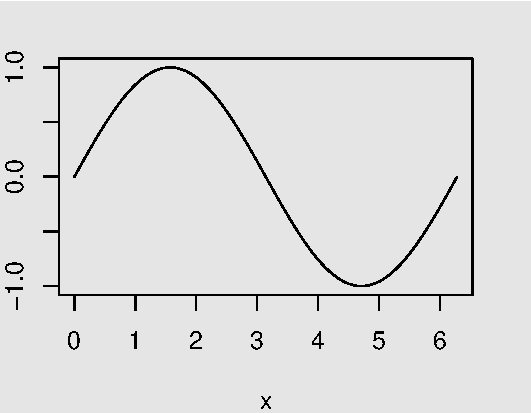
\includegraphics[width=2cm]{media/plot.pdf}! command.

\begin{center}
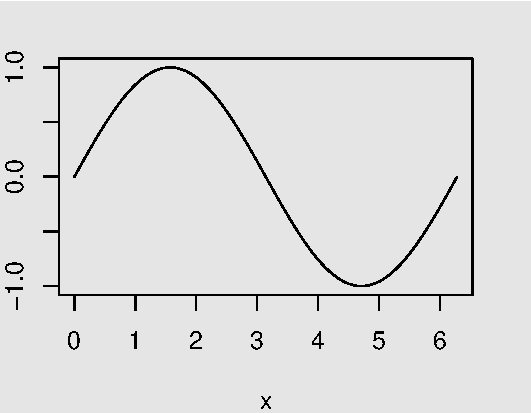
\includegraphics[width=2cm]{media/plot.pdf}
\end{center}

\subsection{The model}

We write inline equations as \(x=x\) or displayed equations as
\begin{equation}\label{eq1}
\mathrm dX_t = \mu\mathrm dt + \sigma\mathrm dB_t
\end{equation}
and reference equations using \lstinline[language=TeX]/\eqref{eq1}/ to display as equation \eqref{eq1}. Maybe we should have added this in \autoref{sec-intro}. You can also reference theorems, for example \lstinline/\autoref{thm:1}/ will produce \autoref{thm:1}.

\begin{definition}
We say that \textbf{$x$ is equal to $x$} whenever $x=x$.
\end{definition}

\begin{lemma}
$x\geq y$ if and only if $y\leq x$.
\end{lemma}
\begin{proof}
This is left as an exercise.
\end{proof}

\begin{proposition}
$x = x$ if and only if $x = x$.
\end{proposition}

\begin{theorem}\label{thm:1}
If $x=x$ and $y=y$, then $x>y$ implies $x>y$.
\end{theorem}

\begin{proof}
A proof with default title.
\end{proof}

\begin{proof}[A proof with custom title]
This is trivial.
\end{proof}

\begin{corollary}
$x>y$ of and only if $y<x$.
\end{corollary}

\begin{remark}
This is a remark.
\end{remark}

\lipsum[2-2]

\section{Results}
You can add tables easily: see \autoref{tab1}. There are three custom column types that accept width specification: \lstinline[]/L/, \lstinline[]/C/ and \lstinline[]/R/, which work similarly to the standard \lstinline[]/p/ column type; for instance, use \lstinline[]/C{4cm}/ for a (horizontally) centered column 4cm wide. Notice, however, that \LaTeX\ has some inconsistencies regarding lengths, as Example \ref{example:lengths} illustrates. Thus, some manual fine-tuning may be necessary to obtain tables with the desired width.

\begin{table}[ht]
\begin{center}
\scalefont{0.9}
\caption{A simple table}\label{tab1}
\begin{tabular}{L{10em}C{5em}c}
\toprule
variable & value & $p$-value\tabularnewline
\midrule
$X$ & 1 & 0.0 \tabularnewline\addlinespace[5pt]
$Y$ & $-1$ & 0.8\tabularnewline
\midrule
{You can write long texts inside\newline table cells, with custom linebreaks} & A & B\tabularnewline
\bottomrule
\end{tabular}
\captionsetup[sub]{width=20em}
\subcaption*{Table descriptions go here. \lipsum[1-1]}
\end{center}
\end{table}



\newpage
\begin{example}\label{example:lengths}
This example illustrates length inconsistencies in \LaTeX.
\begin{table}[ht]
\begin{center}
\rule{.6\textwidth}{1cm}
\begin{tabular}{L{.2\textwidth}C{.2\textwidth}R{.2\textwidth}}
\toprule
a & b & c\tabularnewline\midrule
x & y & z\tabularnewline
\bottomrule
\end{tabular}
\end{center}
\end{table}

The source code yielding the rule and table above is as follows:
\begin{lstlisting}[language = TeX]
\noindent\rule{.6\textwidth}{1cm}
\noindent\begin{tabular}{L{.2\textwidth}C{.2\textwidth}R{.2\textwidth}}
\toprule
x & y & z\tabularnewline\bottomrule
\end{tabular}
\end{lstlisting}
\end{example}

\subsection{Some additional features}
Table~\ref{tab2} illustrates how to align numbers by the decimal place marker. It also shows how to implement the \lstinline[]/\multirow/ command.
\begin{table}[ht]
\begin{center}
\scalefont{0.9}
\caption{Another simple table}\label{tab2}
\begin{tabular}{L{4em}L{4em}r@{.}lc}
\toprule
variable & & \multicolumn{2}{c}{value} & $p$-value\tabularnewline
\midrule
$X$ & & 1&001 & 0.0 \tabularnewline\addlinespace[5pt]
$Y$ & & $-10$&00 & 0.8\tabularnewline\midrule
\multirow{2}{*}{$Z$} & $Z_1$ & 1&1 & 0\tabularnewline
& $Z_2$ & 2&2 & 0\tabularnewline
\bottomrule
\end{tabular}
\end{center}
\end{table}

Here are two useful tools to help formatting \LaTeX\ tables:
\begin{enumerate}[label = (\roman*), itemsep=0pt]
\item \url{https://www.tablesgenerator.com}
\item \url{https://truben.no/table/}
\end{enumerate}
%%%%%%%%%%%%%%%%%%%%%%%%%%%%%%%%%%%%
% END OF DOCUMENT MAIN SECTIONS
%%%%%%%%%%%%%%%%%%%%%%%%%%%%%%%%%%%%


%%%%%%%%%%%%%%%%%%%%%%%%%%%%%%%%%%%%
% ACKNOWLEDGEMENTS
%%%%%%%%%%%%%%%%%%%%%%%%%%%%%%%%%%%%
\paragraph{Acknowledgments}
Author One would like to thank Institution One for financial support.

\paragraph{Conflict of interest} The authors declare no conflict of interest.

\paragraph{Artificial Intelligence} This research utilized AI tools to assist in data analysis, manuscript drafting, and figure generation. All AI-generated content was critically reviewed and validated by the authors to ensure accuracy and alignment with the scientific integrity of the study. The use of AI adhered to ethical guidelines, ensuring transparency and compliance with academic standards. Any biases or limitations inherent to the AI tools were carefully considered in the interpretation of results. The authors affirm that the AI tools did not compromise the originality or integrity of the work.
%%%%%%%%%%%%%%%%%%%%%%%%%%%%%%%%%%%%
% END OF ACKNOWLEDGEMENTS
%%%%%%%%%%%%%%%%%%%%%%%%%%%%%%%%%%%%

%%%%%%%%%%%%%%%%%%%%%%%%%%%%%%%%%%%%
% REFERENCES
%%%%%%%%%%%%%%%%%%%%%%%%%%%%%%%%%%%%
\bibliography{references.bib}\label{refs}
\bibliographystyle{dcu-rbfin}
%%%%%%%%%%%%%%%%%%%%%%%%%%%%%%%%%%%%
% END OF REFERENCES
%%%%%%%%%%%%%%%%%%%%%%%%%%%%%%%%%%%%


%%%%%%%%%%%%%%%%%%%%%%%%%%%%%%%%%%%%

%%%%%%%%%%%%%%%%%%%%%%%%%%%%%%%%%%%%
% APPENDIX
%%%%%%%%%%%%%%%%%%%%%%%%%%%%%%%%%%%%
\rbfinappendix
\section{Matlab Code}

The complete Matlab Code used in this report is listed below: 

loadMNISTImages.m
\begin{lstlisting}
% Load MNIST images from a IDX3-ubyte file
function images = loadMNISTImages(filename)
    % open file with big-endian format
    file = fopen(filename,'r','b');
    % use first 4 bytes to chekc the file type
    if fread(file,1,'int32') ~= 2051
        error('Invalid magic number in %s', filename);
    end
    numImages = fread(file,1,'int32');
    numRows = fread(file,1,'int32');
    numCols = fread(file,1,'int32');
    fprintf('Loading %d images of size %d x %d from %s\n', numImages, numRows, numCols, filename);
    % each pixel is stored as an unsigned byte
    images = fread(file,inf,'unsigned char');
    images = reshape(images, numRows*numCols, numImages);
    images = double(images)/255;
    fclose(file);
    fprintf('Successfully loaded %d images from %s.\n', numImages, filename);
end


\end{lstlisting}

\begin{figure}[ht]
\begin{center}
\caption{Adding subfigures}\label{subfigures}
%
\subcaptionbox{Bivariate Normal with $\rho=1$\label{a}}
{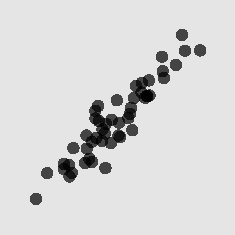
\includegraphics{media/plot2a.pdf}}
%
\subcaptionbox[]{Bivariate Normal with $\rho=0$\label{b}}
{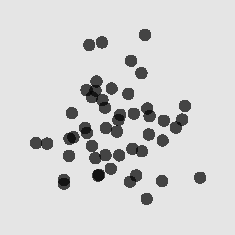
\includegraphics{media/plot2b.pdf}}
%
\end{center}
\end{figure}

\begin{sidewaystable}
\begin{center}
\scalefont{.9}
\caption{A sideways table}\label{tabA1}
\begin{tabular}[]{L{6cm}C{2cm}C{2cm}C{2cm}}
\toprule
\multirow{2}{*}{variable} & \multicolumn{3}{c}{estimation outputs}\tabularnewline
\cmidrule(l){2-4}
& value & $t$-stat. & $p$-value\tabularnewline
\midrule
$X$ & 1 & 3.59 & 0.0 \tabularnewline\addlinespace[5pt]
$Y$ & $-1$ & $-0.1$ & 0.8\tabularnewline
\midrule
{You can write long texts inside\newline table cells, with custom linebreaks} & A & B & C\tabularnewline
\bottomrule
\end{tabular}
\end{center}
\end{sidewaystable}
%%%%%%%%%%%%%%%%%%%%%%%%%%%%%%%%%%%%
% END OF APPENDIX
%%%%%%%%%%%%%%%%%%%%%%%%%%%%%%%%%%%%

\end{document}

%%%%%%%%%%%%%%%%%%%%%%%%%%%%%%%%%%%%
% END OF DOCUMENT
%%%%%%%%%%%%%%%%%%%%%%%%%%%%%%%%%%%%